% 图 7.1 (a) k 空间允许波矢均匀点阵，间距 2π/L (b) k 空间球体、点刻八分楔形与厚 dk 球壳
\documentclass[tikz,border=5pt]{standalone}
\usetikzlibrary{arrows.meta,patterns}
\usepackage{amsmath}
\usepackage{bm}
\usepackage{fontspec}
\setmainfont{Times New Roman}
\begin{document}
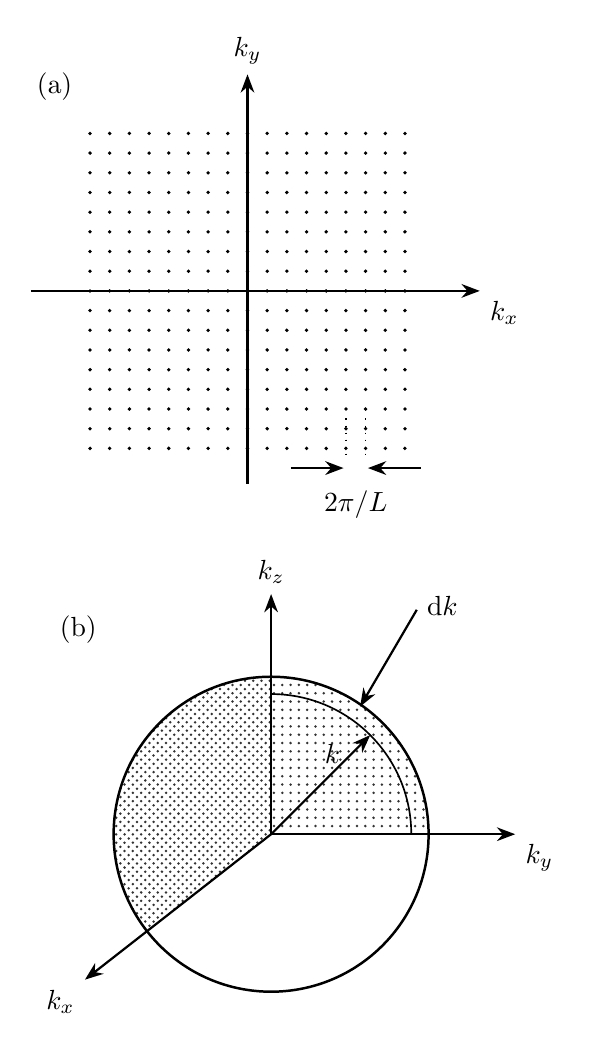
\begin{tikzpicture}[line width=0.8pt,>=Stealth]
% ---------- (a) 点阵 ----------
\begin{scope}
\node at (-2.45,2.6) {(a)};
% 网格点 17x17，间距 0.25
\foreach \i in {-8,...,8}
  \foreach \j in {-8,...,8}
    \fill (\i*0.25,\j*0.25) circle (0.024);
% 坐标轴
\draw[->] (0,-2.45) -- (0,2.75) node[above] {$k_y$};
\draw[->] (-2.75,0) -- (2.95,0) node[below right] {$k_x$};
% 2π/L 标注：两相邻点列的竖直点线 + 相向箭头
\draw[dotted,line width=0.55pt] (1.25,-1.62) -- (1.25,-2.1);
\draw[dotted,line width=0.55pt] (1.5,-1.62) -- (1.5,-2.1);
\draw[->] (0.55,-2.25) -- (1.22,-2.25);
\draw[->] (2.2,-2.25) -- (1.53,-2.25);
\node at (1.375,-2.72) {$2\pi/L$};
\end{scope}
% ---------- (b) 球体 + 八分楔形 + dk 壳 ----------
\begin{scope}[shift={(0.3,-6.9)}]
\node at (-2.45,2.6) {(b)};
% 左侧楔形（k_z 与 k_x 之间，浓点刻）
\path[pattern=crosshatch dots,pattern color=black!80]
  (0,0) -- (0,2) arc (90:218:2) -- cycle;
% 前面八分区（k_z 与 k_y 之间，点刻）
\path[pattern=dots,pattern color=black!80]
  (0,0) -- (0,2) arc (90:0:2) -- cycle;
% 球壳内边界弧（r=k 对应 1.78）
\draw[line width=0.6pt] (1.78,0) arc (0:90:1.78);
% 球轮廓
\draw[line width=0.9pt] (0,0) circle (2);
% 坐标轴
\draw[->] (0,0) -- (0,3.05) node[above] {$k_z$};
\draw[->] (0,0) -- (3.1,0) node[below right] {$k_y$};
\draw[->] (0,0) -- (218:3.0) node[below left] {$k_x$};
% 半径箭头 k（至壳内边界）
\draw[->] (0,0) -- (45:1.78);
\node at (0.78,1.02) {$k$};
% dk 箭头指向壳带
\draw[->] (1.85,2.85) -- (1.13,1.62);
\node[right] at (1.85,2.9) {$\mathrm{d}k$};
\end{scope}
\end{tikzpicture}
\end{document}
